\experiment{Polynomial Linked List}{18/11/2023}

\section{Aim}
To implement a program that performs addition and multiplication on polynomials using linked lists.

\section{Algorithm}
 {\fontfamily{lmtt}\selectfont

  \subsection{Structure Definition}
  Create a structure \texttt{Node} with the following attributes:
  \begin{enumerate}[label=\arabic*:,left=0pt]
    \item Integer \texttt{exp} to store the exponent of the term.
    \item Integer \texttt{coeff} to store the coefficient of the term.
    \item Pointer to \texttt{Node} \texttt{next} for linking nodes.
  \end{enumerate}

  \subsection{Insertion Function}
  Create a function \texttt{insertBegin(head, coeff, exp)}:
  \begin{enumerate}[label=\arabic*:,left=0pt]
    \item \textbf{Start}
    \item Allocate memory for a new \texttt{Node} structure using \texttt{malloc}.
    \item If allocation fails, print "Memory allocation failed" and exit.
    \item Set \texttt{coeff} and \texttt{exp} in the new node.
    \item Set \texttt{next} of the new node to \texttt{head}.
    \item Set \texttt{head} to the new node.
    \item Return the updated \texttt{head}.
    \item \textbf{Stop}
  \end{enumerate}

  \subsection{Bubble Sort Function}
  Create a function \texttt{bubblesort(head, n)}:
  \begin{enumerate}[label=\arabic*:,left=0pt]
    \item \textbf{Start}
    \item Loop from \texttt{i} equal to \texttt{n - 1} down to 0:
          \begin{enumerate}[label=2.\arabic*:, start=1]
            \item Set \texttt{current} to \texttt{head}.
            \item Loop from \texttt{j} equal to 0 to \texttt{i}:
                  \begin{enumerate}[label=2.2.\arabic*:, start=1]
                    \item Set \texttt{next} to \texttt{current->next}.
                    \item If \texttt{current->exp > next->exp}, swap the \texttt{coeff} and \texttt{exp} values.
                    \item Set \texttt{current} to \texttt{next}.
                  \end{enumerate}
          \end{enumerate}
    \item \textbf{Stop}
  \end{enumerate}

  \subsection{Display Function}
  Create a function \texttt{display(head)}:
  \begin{enumerate}[label=\arabic*:,left=0pt]
    \item \textbf{Start}
    \item Set \texttt{current} to \texttt{head}.
    \item Loop while \texttt{current} is not \texttt{NULL}:
          \begin{enumerate}[label=2.\arabic*:, start=1]
            \item If \texttt{current} is not equal to \texttt{head}, print " + ".
            \item Print \texttt{current->coeff} and \texttt{current->exp}.
            \item Set \texttt{current} to \texttt{current->next}.
          \end{enumerate}
    \item Print a newline.
    \item \textbf{Stop}
  \end{enumerate}

  \subsection{Multiply Function}
  Create a function \texttt{multiply(a, b)}:
  \begin{enumerate}[label=\arabic*:,left=0pt]
    \item \textbf{Start}
    \item Set \texttt{result} to \texttt{NULL}.
    \item Set \texttt{currenta} to \texttt{a}.
    \item Set \texttt{n} to 0.
    \item Loop while \texttt{currenta} is not \texttt{NULL}:
          \begin{enumerate}[label=2.\arabic*:, start=1]
            \item Set \texttt{currentb} to \texttt{b}.
            \item Loop while \texttt{currentb} is not \texttt{NULL}:
                  \begin{enumerate}[label=2.2.\arabic*:, start=1]
                    \item Calculate \texttt{coeff} and \texttt{exp} by multiplying \texttt{currenta->coeff} with \texttt{currentb->coeff} \newline and adding \texttt{currenta->exp} with \texttt{currentb->exp}.
                    \item Set \texttt{currentr} to \texttt{result}.
                    \item Set \texttt{alreadyExist} to 0.
                    \item Loop while \texttt{currentr} is not \texttt{NULL}:
                          \begin{enumerate}[label=2.2.3.\arabic*:, start=1]
                            \item If \texttt{currentr->exp == exp}, update \texttt{currentr->coeff} by adding \texttt{coeff} and \newline set \texttt{alreadyExist} to 1.
                            \item Set \texttt{currentr} to \texttt{currentr->next}.
                          \end{enumerate}
                    \item If \texttt{alreadyExist} is 0, increment \texttt{n}, and insert a new node with \texttt{coeff} and \texttt{exp} at the \newline beginning of \texttt{result}.
                  \end{enumerate}
            \item Set \texttt{currentb} to \texttt{currentb->next}.
          \end{enumerate}
    \item Call \texttt{bubblesort(result, n)}.
    \item \textbf{Stop}
  \end{enumerate}

  \subsection{Add Function}
  Create a function \texttt{add(a, b)}:
  \begin{enumerate}[label=\arabic*:,left=0pt]
    \item \textbf{Start}
    \item Set \texttt{result} to \texttt{NULL}.
    \item Set \texttt{currenta} to \texttt{a}.
    \item Set \texttt{currentb} to \texttt{b}.
    \item Set \texttt{n} to 0.
    \item Loop while \texttt{currenta} is not \texttt{NULL} or \texttt{currentb} is not \texttt{NULL}:
          \begin{enumerate}[label=2.\arabic*:, start=1]
            \item If \texttt{currenta} and \texttt{currentb} are not \texttt{NULL}:
                  \begin{enumerate}[label=2.2.\arabic*:, start=1]
                    \item If \texttt{currenta->exp == currentb->exp}, calculate \texttt{coeff} by adding \texttt{currenta->coeff} and \newline \texttt{currentb->coeff} and insert a new node with \texttt{coeff} and \texttt{currenta->exp} at the \newline beginning of \texttt{result}.
                    \item Move \texttt{currenta} and \texttt{currentb} to their next nodes.
                  \end{enumerate}
            \item If only \texttt{currenta} is not \texttt{NULL}, insert a new node with \texttt{currenta->coeff} and \texttt{currenta->exp} \newline at the beginning of \texttt{result}.
            \item If only \texttt{currentb} is not \texttt{NULL}, insert a new node with \texttt{currentb->coeff} and \texttt{currentb->exp} \newline at the beginning of \texttt{result}.
            \item Increment \texttt{n}.
          \end{enumerate}
    \item Call \texttt{bubblesort(result, n)}.
    \item \textbf{Stop}
  \end{enumerate}

  \subsection{Main Function}
  In the \texttt{main} function:
  \begin{enumerate}[label=\arabic*:, start=1]
    \item \textbf{Start}
    \item Declare \texttt{a} and \texttt{b} as \texttt{NULL}.
    \item Declare integers \texttt{n1} and \texttt{n2}.
    \item Print "Enter the number of terms of a: ".
    \item Take user input for \texttt{n1} and insert nodes at the beginning of \texttt{a} with user-input \newline coefficients and exponents.
    \item Print "Enter the number of terms of b: ".
    \item Take user input for \texttt{n2} and insert nodes at the beginning of \texttt{b} with user-input \newline coefficients and exponents.
    \item Call \texttt{bubblesort(a, n1)} and \texttt{bubblesort(b, n2)}.
    \item Print "a = " and \texttt{display(a)}.
    \item Print "b = " and \texttt{display(b)}.
    \item Call \texttt{multiply(a, b)} and assign the result to \texttt{product}.
    \item Print "Product = " and \texttt{display(product)}.
    \item Call \texttt{add(a, b)} and assign the result to \texttt{sum}.
    \item Print "Sum = " and \texttt{display(sum)}.
    \item \textbf{Stop}
  \end{enumerate}
 }

\section{C Program}
\begin{lstlisting}[label={list:c_program:polynomial_operations}]
#include <stdlib.h>
#include <stdio.h>

typedef struct Node
{
  int exp;
  int coeff;
  struct Node *next;
} node;

node *insertBegin(node *head, int coeff, int exp);
void display(node *head);
void bubblesort(node *head, int n);
node *multiply(node *a, node *b);
node *add(node *a, node *b);

int main()
{
  node *a = NULL;
  node *b = NULL;
  int n1, n2;
  printf("Enter the number of terms of a: ");
  scanf("%d", &n1);
  for (int i = 0; i < n1; i++)
  {
    printf("\nEnter coefficient and exponents: ");
    int c, e;
    scanf("%d %d", &c, &e);
    a = insertBegin(a, c, e);
  }

  printf("\nEnter the number of terms of b: ");
  scanf("%d", &n2);
  for (int i = 0; i < n2; i++)
  {
    printf("\nEnter coefficient and exponents: ");
    int c, e;
    scanf("%d %d", &c, &e);
    b = insertBegin(b, c, e);
  }
  bubblesort(a, n1);
  bubblesort(b, n2);
  printf("a = ");
  display(a);
  printf("b = ");
  display(b);
  node *product = multiply(a, b);
  printf("Product = ");
  display(product);
  node *sum = add(a, b);
  printf("Sum = ");
  display(sum);
}

node *insertBegin(node *head, int coeff, int exp)
{
  node *temp = NULL;
  temp = (node *)malloc(sizeof(node));
  if (temp == NULL)
  {
    printf("Memory allocation failed");
    exit(0);
  }
  temp->coeff = coeff;
  temp->exp = exp;
  temp->next = head;
  head = temp;
  return head;
}

void bubblesort(node *head, int n)
{
  for (int i = n - 1; i >= 0; i--)
  {
    node *current = head;
    for (int j = 0; j < i; j++)
    {
      node *next = current->next;
      if (current->exp > next->exp)
      {
        int texp = current->exp;
        int tcoeff = current->coeff;
        current->coeff = next->coeff;
        current->exp = next->exp;
        next->coeff = tcoeff;
        next->exp = texp;
      }
      current = next;
    }
  }
}

void display(node *head)
{
  node *current = head;
  while (current != NULL)
  {
    if (current != head)
      printf(" + ");
    printf("%dx^%d", current->coeff, current->exp);
    current = current->next;
  }
  printf("\n");
}

node *multiply(node *a, node *b)
{
  node *result = NULL;
  node *currenta = a;
  int n = 0;
  while (currenta != NULL)
  {
    node *currentb = b;
    while (currentb != NULL)
    {
      int coeff = currenta->coeff * currentb->coeff;
      int exp = currenta->exp + currentb->exp;
      node *currentr = result;
      int alreadyExist = 0;
      while (currentr != NULL)
      {
        if (currentr->exp == exp)
        {
          currentr->coeff += coeff;
          alreadyExist = 1;
        }
        currentr = currentr->next;
      }
      if (!alreadyExist)
      {
        n++;
        result = insertBegin(result, coeff, exp);
      }
      currentb = currentb->next;
    }
    currenta = currenta->next;
  }
  bubblesort(result, n);
  return result;
}

node *add(node *a, node *b)
{
  node *result = NULL;
  node *currenta = a;
  node *currentb = b;
  int n = 0;
  while (currenta != NULL || currentb != NULL)
  {
    if (currenta != NULL && currentb != NULL)
    {
      if (currenta->exp == currentb->exp)
      {
        int coeff = currenta->coeff + currentb->coeff;
        result = insertBegin(result, coeff, currenta->exp);
        currenta = currenta->next;
        currentb = currentb->next;
      }
      else if (currenta->exp < currentb->exp)
      {
        result = insertBegin(result, currenta->coeff, currenta->exp);
        currenta = currenta->next;
      }
      else
      {
        result = insertBegin(result, currentb->coeff, currentb->exp);
        currentb = currentb->next;
      }
      n++;
    }
    else if (currenta != NULL)
    {
      result = insertBegin(result, currenta->coeff, currenta->exp);
      currenta = currenta->next;
      n++;
    }
    else if (currentb != NULL)
    {
      result = insertBegin(result, currentb->coeff, currentb->exp);
      currentb = currentb->next;
      n++;
    }
  }
  bubblesort(result, n);
  return result;
}
\end{lstlisting}

\section{Output}
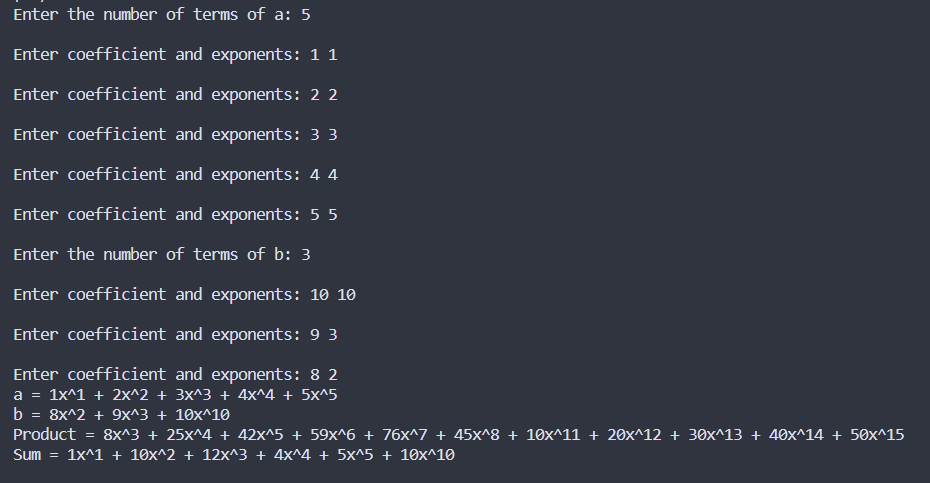
\includegraphics[width=\textwidth]{Cycle_2/Outputs/Polynomial.png}

\section{Result}
Program is executed and the output is verified